%!TEX root = thesis.tex
As a way of introduction we will here give an overview of the evolution of computer interfaces and how they have interacted and integrated with the users using them.
We will use this a starting point as to situate ourself in relation to the various fields of research in computer science and as a pointer to the future prospects of user interfaces, both in terms of what visions other researchers have proposed, and in relation to our own proposition for ad hoc interfaces.
We will first give a historical look back in time based on \citet{grudin1990computer}, from the early computers to the 1990s, which will both give an insight as to how the relationship between the user and computers has evolved, as well as point to a paradigm shift away from the terminal based computer.
We will follow this paradigm shift to the vision of ubiquitous computer, presented by \citet{weiser1991computer}, and look at some of the relevant related research area that has followed this vision.
Lastly we will point to an area where we see unused potential for future work, an area that throughout this thesis will be further articulated and conceptualized.   

\section{The computer reaches out}
There is of course many ways to look at the evolution of the computer and the user interface, and although it is hard to draw a straight line as to how the development has occurred, as much of the developments has happened in parallel, we try to outline the broad picture and give a pointer to the future.
As a start we have chosen to take an offset in \citeauthor{grudin1990computer}'s article about the historical continuity of interface design \citep{grudin1990computer} and along with that, the type of interaction that has been defining for each of \citeauthor{grudin1990computer}'s levels.

\citeauthor{grudin1990computer} describes the evolution of the user interface from the 1950's to the 1990's though five overall development foci or 'levels' for researchers, along with the principle user group for each level.
The five levels can be seen visualized in figure~\ref{foci-interface}.

\begin{figure}[hb]
	\centering
  		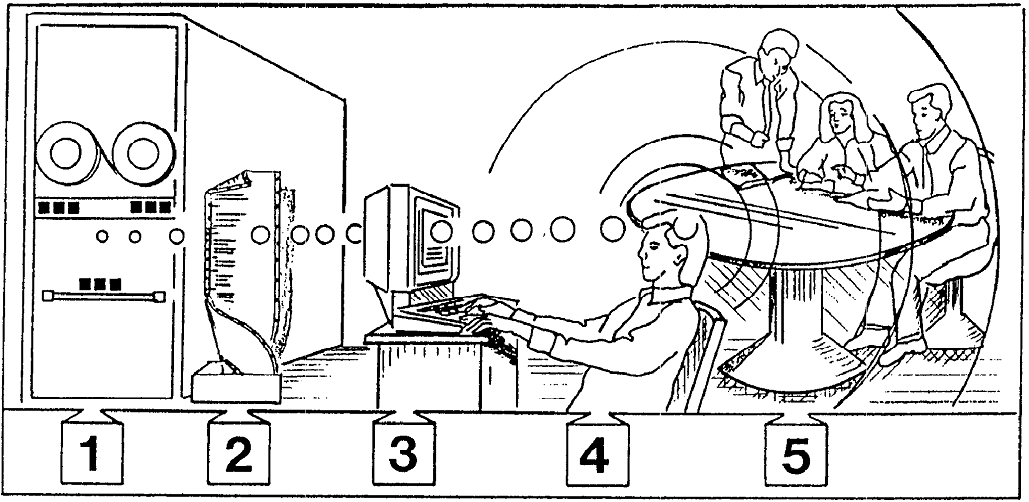
\includegraphics[width=3in]{figures/foci-interface}
	\caption[The development of user interfaces \citep{grudin1990computer}.]
   {The development of user interfaces, from \citep{grudin1990computer}.}
   \label{foci-interface}
\end{figure}
The levels should not be seen as isolated entities, as there exists interdependencies between the levels, for example before progress can be made to level 2, there might have to be made improvements to the hardware at level 1.

\subsubsection{Level 1: Interface as hardware}
At the first level (-1950s) the interface is seen as hardware, understood in the way that the interaction between the user and the computer is defined by the workings of the hardware.
So for engineers and programmers, which are the principal users, a central part of the user interaction involves the inner workings of the hardware.
A common way to interact at the time were, besides modifying the hardware, was though punch cards.
Punch cards represents digital information by the presence or absence of holes on the card, based on a predefined pattern which the computer can then read.
The user would use a machine to punch holes in the cards which could contain programming commands or it could be used as an analogue data storage that could later be read by the computer.
From a human perspective the interaction at the time was very much on the premises of the computer, as the language of interaction was based on things like binary numbers, hexadecimals and memory locations.

\subsubsection{Level 2: Interface as software}
The second level (1960s-1970s) defines the interface as software.
As the hardware level is abstracted away by advancements in software and programming languages programmers and the interface they interacts with moves away from the physical inner workings of the computer and onto software.
The main users now mostly programmers and the interface focus is on the computer, so the user interaction is still on the premises of the computer, with a lack of attention to human factors like legibility of code.
Programmers interacted with the computer though assembly code, compilers and mathematics as the main focus of the computer was on computations. The notion of a \emph{user interface} was still unarticulated as interface development was focused on programmer efficiency, not human factors.

\subsubsection{Level 3: Interface as terminal}
At the third level (1970s-1990s) the interface focus moves away from the programming task and onto the terminal where the dominant user is no longer necessarily programmers or engineers, but seen more broadly as \emph{end-users}.
Grundin also marks this as the start of the discipline of human-computer interaction, including the `human' in the computer interaction.
The move to the terminals was made possible by advances in visual displays and interactive capabilities, letting the user, to a larger degree than before, interact on more human terms where the interface aids the user in the interaction.

With the emergence of the computer mice and more powerful computers, Graphical User Interfaces (GUIs) became, and still is, the most popular method of interacting with the computer.
One of the main aspects of the GUI is the use of visual metaphors, inspired by the real world, to guide the users actions and understanding of the system.
The most well knows being the desktop metaphor that links the office space to the computer with digital folders, documents, trash bins and so on, simulating a physical desktop on the monitor.
The central components of the desktop metaphor being windows, icons, menus and pointers, also known as the WIMP paradigm \citep[chap. 6]{krumm2009ubiquitous}. 
Using metaphors in this way can ease the user's annexation into the digital world as they, if done properly, creates logical links between knows physical actions and potential digital actions.

\subsubsection{Level 4: Interface as dialogue}
The use of metaphors as described in level 3 does also somewhat fit into the this level since the GUI, in the previous example, is adapting physical attributes (the office) into the virtual space and in that way incorporates the surrounding environment, though in a static way.
The fourth level (1980s-) focus on the interface as an interaction dialogue where the interface can be adapted and tailored, by the computer, to the specific user.
This could for example be computer systems, over time, gathers information about the users interaction patterns enabling it to possibly foresee a user action, and maybe by making it easier to execute the action, assisting the user.
Grundin sees it as the computer \emph{``is extending its grasp beyond the keyboard and the display surface''} in the sense that the computer now has some knowledge about the user which lets it partake in a two-way dialogue.

\subsubsection{Level 5: Interface as work setting}
The fifth level (1990s-) takes the interaction dialogue to the work or social setting, moving the interface further away from the computer.
The principal user is now a group of ``end-users'' and as the interaction takes place in a social setting it is increasingly necessary for the computer to have information about the surrounding environment.
Social settings are generally complex structures where environment, culture, social structures, group dynamics, and context all play a role in the dynamics of social interaction.
All of these aspects needs, to some degree, to be design for in a user interface aimed at the work or social setting, increasing the complexity of the system.
\blank
Grundins five levels describes a movement where the interface separates itself from the physical enclosure of the hardware and into the cognitive and social structures of humans.
\citeauthor{grudin1990computer} himself describes it as a continuously \emph{``outward movement of the computer's interface to its external environment''}.
A concequence of this is that a move in the interaction language also happens, from abstract to natural, in terms of the human readability, as the focus of the interface moves from the computer to its user.

Grundin points out that as of 1990 most work has been focused on the third level but he sees a future where the interface dialogue and the social setting is increasingly influential in the design of computing systems.
This notion is not far away from what \citeauthor{weiser1991computer} presents a year later in his vision of ubiquitous computing \citep{weiser1991computer}.

\subsection{Ubiquitous computing}
In traditional computer systems there has generally been a strong separation between the physical and the digital, but with ubiquitous computing, not only does the computer's interface move to its external environment, as Grundin pointed to, we also see that the computer itself moves into the environment, creating a stronger link between the physical world and the digital world.
A consequence of ubiquitous computing is also a change in the relationship between the user and computers.
This change can be seen by looking at the evolution of the relationship, which can be roughly split into three generations or eras \citep{weiser1997coming,abowd2012next}.
\begin{itemize}
\item[] \textbf{1\textsuperscript{st} generation} being terminal based computing where multiple users share the same computer in a many-to-one relationship.
\item[] \textbf{2\textsuperscript{nd} generation} where the personal computing revolution happens and it becomes possible to have \emph{your} computer, in a one-to-one relationship between the computer and the user.
\item[] \textbf{3\textsuperscript{rd} generation} being ubiquitous computing, here a one-to-many relationship becomes possible as computers move out into the world and multiple computers now shares and interacts with a single person.
\end{itemize}

The idea of ubiquitous computing, as presented in \citep{weiser1991computer}, is that a multitude of interconnected computers are embedded seamlessly into the environment as to become invisible, both physical and metaphorical, and integrate into the everyday life of people.
In contrast to terminal based computing, interactions with these systems can happen everywhere, with a multitude of different devices with computers with many different forms. 
This points to two key aspects of attaining this vision, \emph{location} and \emph{scale}.
The purpose of location is to be able to inform the user and adapt to the need of the user based on the location context available to system. 
The aspect of scale is relevant for creating \emph{``machines that fit the human environment, instead of
forcing humans to enter their''}, as \citeauthor{weiser1991computer} puts it, where different sized computers can fit into different environments, contexts or functions. 

This vision of moving a multitude of computers and their user interface out into the world has been the basis inspiration for an array of related research areas, each with a specific focus or approach, but with the shared purpose of going beyond the situated use of the desktop computer, and its WIMP interface, and move into the environment.

We will limit ourself to present only a selected few areas following the ubiquitous vision that we find relevant to our own work and which will be further discussed throughout the thesis.
\subsubsection{Context Awareness (CA)}
As mentioned a key part of ubiquitous computing is location and this has laid the basis for the research area of context awareness.
There has been many definition of context and context aware computing, the first being by \citet{schilit1994context}, but here we will stick to the definition proposed by \citeauthor{abowd1999towards} as we find it more encompassing. 

\citet{abowd1999towards} defines context-aware computing as \emph{``the use of context to
provide task-relevant information and/or services to a user''}, where context is \emph{``any information that can be used characterize the situation of an entity''} and entity describing anything that is relevant for the application or user.
\citeauthor{abowd1999towards} describe the control loop of CA applications as three-parted. 
First the application looks at the incoming context, this is the \emph{who's, where's, when's and what's} and based on this information decides on a \emph{why} the situation is occurring and when the \emph{why} is decided, the application should act accordingly with an appropriate \emph{action}
One of the main challenges of making such systems is to define which parts of the context that is relevant in a given situation and how it should translate into a \emph{why}, as this is something that the application designer as to encode into the application.

\subsubsection{Tangible User Interfaces (TUI)}
TUIs attempts to create physical representations of the digital state of the computer, embedding a digital layer into physical objects and environments.
The term was first coined by \citet{ishii1997tangible}, building on Weiser's vision of the ubiquitous and invisible computer.
Ishii and Ullmer states two goals for TUIs:
\begin{itemize}
    \item{allowing users to ``grasp and manipulate'' foreground bits by coupling bits with physical objects, and}
    \item{enabling users to be aware of background bits at the periphery using ambient media in an augmented space}
\end{itemize}
By embodying digital information into tangible objects, TUI systems takes advantage of humans ability to sense, interact and manipulate the physical world. 


\section{A possible future for user interfaces}
\todo{not done at all}
As Abowd correctly notes, Weiser's vision has to some extend become reality. 
Computers are part of the environment and have indeed been \textit{woven} into the fabric of everyday life in many ways. \todo{giv nogle simple eksempler} 
If we are beginning to pass the 3\textsuperscript{rd}, Abowd asks \textit{so, what's next?}.
This is of course a complex and difficult question to answer.
Abowd suggests a future where the human-computer experience is more conjoined than ever, blurring the boundaries between them.
\begin{quote}
\emph{[\ldots] our own physical being and our sense of identity is no longer easily distinguished from elements of computing.}
\end{quote}
Abowd also touches on a topic that has been dominant in the last few years, namely cloud computing.
Broadly seen cloud computing refers to services and applications that are made available over a network \todo{wiki ref?}.
This could be data storage, computing power, back-up services or applications which makes traditional desktop applications available through the Internet.
Abowd suggests that future devices will be able to adapt to whoever is currently using it, as all relevant information will available be in from the cloud.
Following this, devices and their services no longer have to be closely ties together, leading the way for genetic multi purpose devices that delivers services from the cloud.

\citet{ishii2012radical} presents an alternative vision for the future.
They presents the vision as \textit{Radical Atoms}, a vision for the future of \textit{human-material interaction} or \textit{material user interface}. 

\todo{noget med shape change - ledende op til SC afsnit og vores protype og ide om ad hoc interfaces}
\todo{3.wave HCI bødker}